\documentclass{beamer}
\usepackage[utf8]{inputenc}
\usepackage[T1]{fontenc}
\usepackage[ngerman]{datetime}
\usepackage{pgfplots} % 
%\usepgfplotslibrary{external} % externalize plots so they don't recompile each time
%\tikzexternalize
\pgfplotsset{width=\textwidth,compat=1.16}
\usepackage{colortbl} % colors for tables
\renewcommand{\dateseparator}{.} % use dots instead of slashes to seperate dates
\usetheme{thk}
% custom colors:
% thk-red
% thk-orange
% thk-violet
% thk-red-0 to thk-red-9 give gradients from red to white, where 9 is almost all white
% the same applies to all colors


\title{\LaTeX -Beamer Theme TH Köln}
\subtitle[Beispielpräsi]{Eine Beispielpräsentation}
\institute[TH Köln]{Technische Hochschule Köln}
% if a short version is given, the footer will preferably use it. If you don't provide a short version in brackets, only the long version will be used.
\supervisor{\insertinstitute} %leave empty if not applicable or
	% use this tag for different purposes, e.g. to provide your email address
\date[\ddmmyyyydate\today]{\today} %short date in brackets, long date in braces
\author{Markus de Koster}
\pagefooterlocalization{Seite } % can be anything, e.g. "Slide" "Page" "Seite"

\begin{document}

% Title page
\begin{frame}
    \vspace{2em} %some distance to the top
    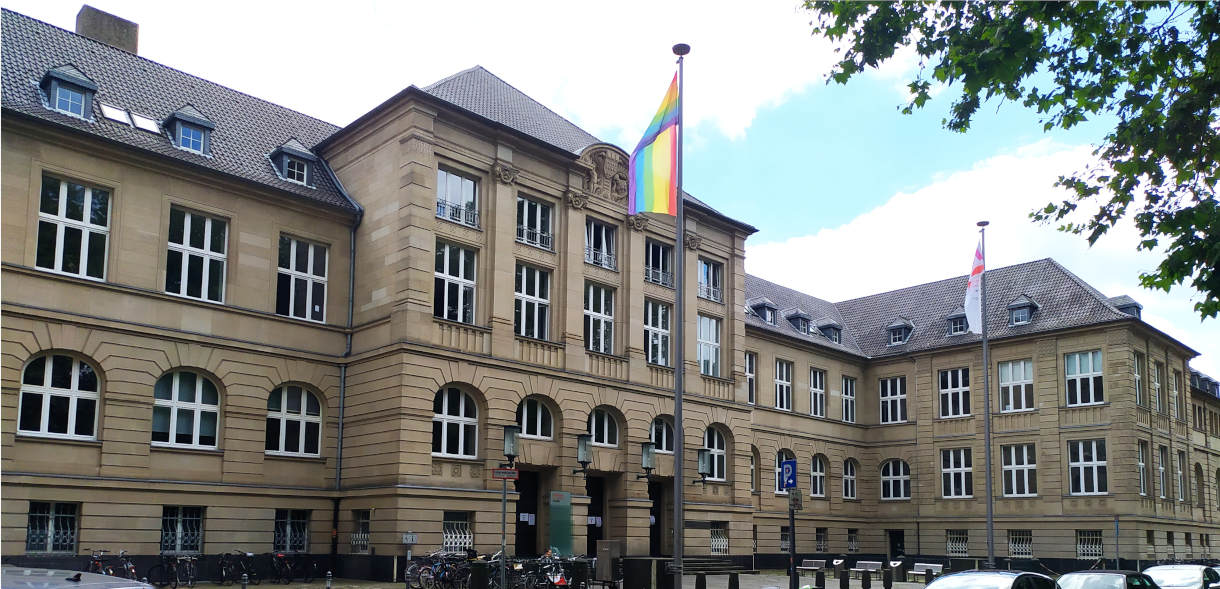
\includegraphics[width=\textwidth]{figures/thk.jpg}
    \titlepage
\end{frame}

% Table of Contents
\begin{frame}
    \frametitle{Inhalt}
    \tableofcontents
\end{frame}

% First slide
\section{Aufzählungen}\label{sec:enumerations} % Sections are used for Table of Contents, Labels can be used for references to this section
\begin{frame} 
    \frametitle{Aufzählungen} 
    \framesubtitle{Ein Beispiel für Aufzählungen} 
    \begin{enumerate} 
        \item item 
        \begin{enumerate} 
            \item subitem
            \begin{enumerate} 
                \item subsubitem
            \end{enumerate}
        \end{enumerate}
        \item item
    \end{enumerate}
\end{frame}

\subsection*{Bulletpoints}\label{sec:itemize}
\begin{frame}[allowframebreaks]{Bulletpoints}
    \begin{itemize}
        \item Die erste Stufe ist in rot
        \begin{itemize}
            \item die zweite in orange
            \begin{itemize}
                \item die dritte in Violet
                \item mehr als drei mal darf nicht indentiert werden
            \end{itemize}    
            \item Die Schrift wird je Stufe etwas kleiner
        \end{itemize}    
        \item Weitere bulletpoints haben die selbe Farbe
        \item Dadurch, dass am Beginn dieses Frames das Attribut "allowframebreaks" gesetzt wurde, wird automatisch eine neue Slide geöffnet, wenn diese voll ist
        \begin{itemize}
            \item dafür müssen wir allerdings den "itemize" Bereich verlassen
            \item \dots
        \end{itemize}
    \end{itemize}
    Wenn die Slide voll ist, wird dieser Text auf die nächste Seite geschoben.
    Dadurch wird automatisch im Titel der Seite ein Zähler eingefügt. 
    Innerhalb eines itemize erfolgt kein Seitenumbruch. 
    Stattdessen werden die items skaliert. 
    Das selbe gilt für Grafiken, Tabellen, etc.
\end{frame}

% colors for table columns
\newcolumntype{v}{>{\columncolor{thk-violet-9}}c}

\section{Tabellen}\label{sec:tables}
\begin{frame} 
    \frametitle{Tabellen} 
    \begin{table}[ht]
        \centering
        \begin{tabular}{ v|l|l } 
          \rowcolor{thk-violet-6}
          \textbf{Name} & \textbf{Anzahl Bytes} & \textbf{Anzahl Bits} \\ 
          \hline
          SHA-1 &  20 & 160 \\ 
          \hline
          SHA-256 &  32 & 256 \\ 
          \hline
          SHA-512 &  64 & 512 \\ 
          \hline
          MD5 &  16 & 128 \\ 
        \end{tabular}
        \caption{\label{tab:example_table} Eine simple Beispieltabelle}
    \end{table}

\end{frame}

\section{Grafiken}\label{sec:graphics}
\begin{frame}{Grafiken}
    \begin{figure}\label{thk-linien}
        
\includegraphics[width=\textwidth]{figures/thk-lines.png}
        \caption[TH Köln lines]{TH Köln lines. Adaptiert von \cite{source}}
    \end{figure}
\end{frame}

\section{Blöcke und Theoreme}\label{sec:block}
\begin{frame} 
    \frametitle{Blöcke und Theoreme} 
    \begin{theorem}
        Theoreme heißen immer Theorem und werden in Violet angezeigt.
    \end{theorem}
	
	\begin{variableblock}{Variabler Block}{bg=thk-red-8, fg=black}{bg=thk-red, fg=white}
		Farbe und Titel von Variablen Blöcken können manuell gesetzt werden
	\end{variableblock}

    \begin{variableblock}{Variabler Block anderer Farbe}{bg=thk-orange-8, fg=black}{bg=thk-orange, fg=white}
        Inline Math: $\int_2^3 x^2 \, dx=\frac{3^3}{3}-\frac{2^3}{3}=\frac{19}{3}$
    \end{variableblock}
\end{frame}

\section{Spalten}\label{sec:columns}
\begin{frame} 
    \frametitle{Spalten} 
    \begin{columns}
        \begin{column}{0.5\textwidth}
            \begin{itemize}
                \item Um mehrere Spalten zu erstellen, muss zuerst die columns Umgebung betreten werden
                \item Danach kann die Spaltengröße für jede Spalte einzeln gesetzt werden
                \item Sie sollte insgesamt die Textweite nicht übersteigen
            \end{itemize}
        \end{column}
        \begin{column}{0.5\textwidth}
            \begin{center}
                \begin{figure}\label{thk-claudiusstr}
                    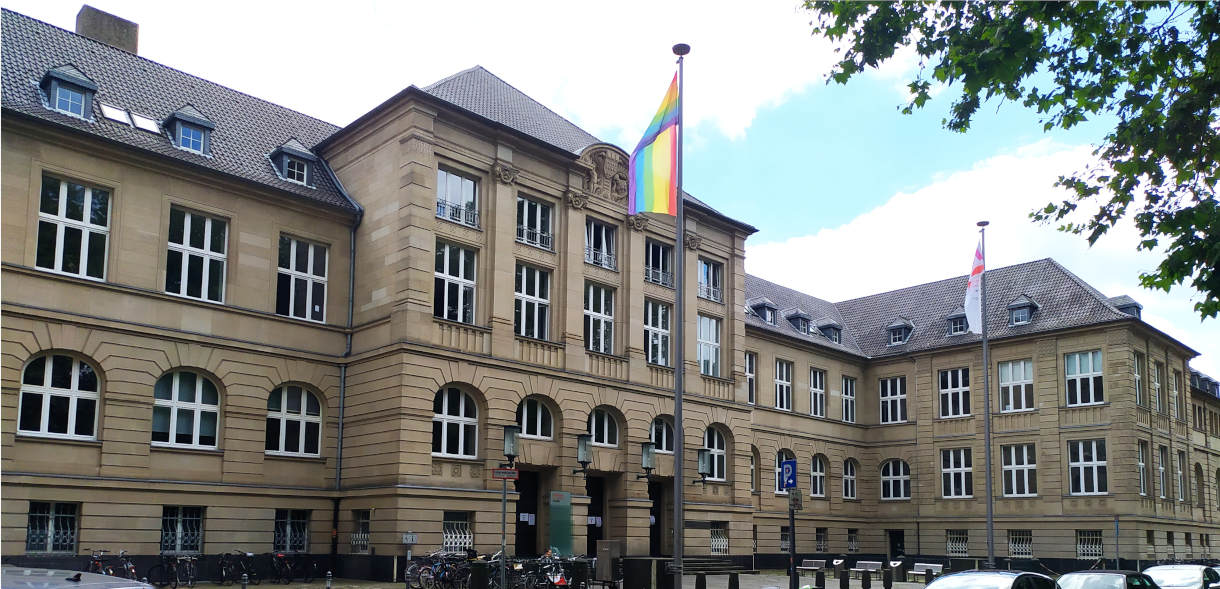
\includegraphics[width=\textwidth]{figures/thk.jpg}
                    \caption[TH Köln Claudiusstr.]{TH Köln Claudiusstraße 1. Quelle: eigene Aufnahme}
                \end{figure}
            \end{center}
        \end{column}    
    \end{columns}
    
    
\end{frame}

\section{Plots}\label{sec:plots}
\begin{frame} 
    \frametitle{Plots} 
    \begin{columns}
        \begin{column}{0.5\textwidth}
            \begin{figure}\label{2dPlot}
                \begin{tikzpicture}
                    \begin{axis}
                    \addplot[color=thk-red]{exp(x)};
                    \addplot[color=thk-violet]{-2*x^2+ 50};
                    \end{axis}
                \end{tikzpicture}
                \caption[2D Plot]{2D Plot using pgfplots}
            \end{figure}
        \end{column}
        \begin{column}{0.5\textwidth}
            \begin{figure}\label{3dPlot}
                \begin{tikzpicture}
                    \begin{axis}
                    \addplot3[
                        surf,
                        colormap={rw}{color=(thk-red) color=(white)},
                        samples=50, samples y=30,
                        domain=-3.5:3.5,domain y=-1:1
                    ]
                    {((x+sin(deg(x)))^2};
                    \end{axis}
                \end{tikzpicture} 
                \caption[3D Plot]{3D Plot using pgfplots and custom color map}
            \end{figure}
        \end{column}    
    \end{columns}       
\end{frame}

\end{document}
